% To disable outputting page headers and footers, remove "runningheads"
\documentclass[runningheads,a4paper,english]{llncs}[2022/01/12]
\usepackage{upquote}
\usepackage[ngerman,main=english]{babel}

\addto\extrasenglish{\languageshorthands{ngerman}\useshorthands{"}}
%
% Fix by https://tex.stackexchange.com/a/441701/9075
\usepackage{regexpatch}
\makeatletter
\edef\switcht@albion{%
  \relax\unexpanded\expandafter{\switcht@albion}%
}
\xpatchcmd*{\switcht@albion}{ \def}{\def}{}{}
\xpatchcmd{\switcht@albion}{\relax}{}{}{}
\edef\switcht@deutsch{%
  \relax\unexpanded\expandafter{\switcht@deutsch}%
}
\xpatchcmd*{\switcht@deutsch}{ \def}{\def}{}{}
\xpatchcmd{\switcht@deutsch}{\relax}{}{}{}
\edef\switcht@francais{%
  \relax\unexpanded\expandafter{\switcht@francais}%
}
\xpatchcmd*{\switcht@francais}{ \def}{\def}{}{}
\xpatchcmd{\switcht@francais}{\relax}{}{}{}
\makeatother

\usepackage[hyphens]{url}

% When activated, use text font as url font, not the monospaced one.
% For all options see https://tex.stackexchange.com/a/261435/9075.
% \urlstyle{same}

% Improve wrapping of URLs - hint by http://tex.stackexchange.com/a/10419/9075
\makeatletter
\g@addto@macro{\UrlBreaks}{\UrlOrds}
\makeatother

% nicer // - solution by http://tex.stackexchange.com/a/98470/9075
% DO NOT ACTIVATE -> prevents line breaks
%\makeatletter
%\def\Url@twoslashes{\mathchar`\/\@ifnextchar/{\kern-.2em}{}}
%\g@addto@macro\UrlSpecials{\do\/{\Url@twoslashes}}
%\makeatother

% This is the modern package for "Computer Modern".
% In case this gets activated, one has to switch from cmap package to glyphtounicode (in the case of pdflatex)
\usepackage[%
    rm={oldstyle=false,proportional=true},%
    sf={oldstyle=false,proportional=true},%
    % By using 'variable=true' the monospaced font can be used as variable font (with differents widths per letter)
    % However, this makes listings look ugly.
    tt={oldstyle=false,proportional=true,variable=false},%
    qt=false%
]{cfr-lm}

% Has to be loaded AFTER any font packages. See https://tex.stackexchange.com/a/2869/9075.
\usepackage[T1]{fontenc}

% Character protrusion and font expansion. See http://www.ctan.org/tex-archive/macros/latex/contrib/microtype/

\usepackage[
  babel=true, % Enable language-specific kerning. Take language-settings from the languge of the current document (see Section 6 of microtype.pdf)
  expansion=alltext,
  protrusion=alltext-nott, % Ensure that at listings, there is no change at the margin of the listing
  final % Always enable microtype, even if in draft mode. This helps finding bad boxes quickly.
        % In the standard configuration, this template is always in the final mode, so this option only makes a difference if "pros" use the draft mode
]{microtype}

% \texttt{test -- test} keeps the "--" as "--" (and does not convert it to an en dash)
\DisableLigatures{encoding = T1, family = tt* }

%\DeclareMicrotypeSet*[tracking]{my}{ font = */*/*/sc/* }%
%\SetTracking{ encoding = *, shape = sc }{ 45 }
% Source: http://homepage.ruhr-uni-bochum.de/Georg.Verweyen/pakete.html
% Deactiviated, because does not look good

\usepackage{graphicx}

% Diagonal lines in a table - http://tex.stackexchange.com/questions/17745/diagonal-lines-in-table-cell
% Slashbox is not available in texlive (due to licensing) and also gives bad results. Thus, we use diagbox
\usepackage{diagbox}

\usepackage{xcolor}

% Code Listings
\usepackage{listings}

\definecolor{eclipseStrings}{RGB}{42,0.0,255}
\definecolor{eclipseKeywords}{RGB}{127,0,85}
\colorlet{numb}{magenta!60!black}

% JSON definition
% Source: https://tex.stackexchange.com/a/433961/9075

\lstdefinelanguage{json}{
    basicstyle=\normalfont\ttfamily,
    commentstyle=\color{eclipseStrings}, % style of comment
    stringstyle=\color{eclipseKeywords}, % style of strings
    numbers=left,
    numberstyle=\scriptsize,
    stepnumber=1,
    numbersep=8pt,
    showstringspaces=false,
    breaklines=true,
    frame=lines,
    % backgroundcolor=\color{gray}, %only if you like
    string=[s]{"}{"},
    comment=[l]{:\ "},
    morecomment=[l]{:"},
    literate=
        *{0}{{{\color{numb}0}}}{1}
         {1}{{{\color{numb}1}}}{1}
         {2}{{{\color{numb}2}}}{1}
         {3}{{{\color{numb}3}}}{1}
         {4}{{{\color{numb}4}}}{1}
         {5}{{{\color{numb}5}}}{1}
         {6}{{{\color{numb}6}}}{1}
         {7}{{{\color{numb}7}}}{1}
         {8}{{{\color{numb}8}}}{1}
         {9}{{{\color{numb}9}}}{1}
}

\lstset{
  % everything between (* *) is a latex command
  escapeinside={(*}{*)},
  %
  language=json,
  %
  showstringspaces=false,
  %
  extendedchars=true,
  %
  basicstyle=\footnotesize\ttfamily,
  %
  commentstyle=\slshape,
  %
  % default: \rmfamily
  stringstyle=\ttfamily,
  %
  breaklines=true,
  %
  breakatwhitespace=true,
  %
  % alternative: fixed
  columns=flexible,
  %
  numbers=left,
  %
  numberstyle=\tiny,
  %
  basewidth=.5em,
  %
  xleftmargin=.5cm,
  %
  % aboveskip=0mm,
  %
  % belowskip=0mm,
  %
  captionpos=b
}

% Enable Umlauts when using \lstinputputlisting.
% See https://stackoverflow.com/a/29260603/873282 für details.
% listingsutf8 did not work in June 2020.
\lstset{literate=
  {á}{{\'a}}1 {é}{{\'e}}1 {í}{{\'i}}1 {ó}{{\'o}}1 {ú}{{\'u}}1
  {Á}{{\'A}}1 {É}{{\'E}}1 {Í}{{\'I}}1 {Ó}{{\'O}}1 {Ú}{{\'U}}1
  {à}{{\`a}}1 {è}{{\`e}}1 {ì}{{\`i}}1 {ò}{{\`o}}1 {ù}{{\`u}}1
  {À}{{\`A}}1 {È}{{\'E}}1 {Ì}{{\`I}}1 {Ò}{{\`O}}1 {Ù}{{\`U}}1
  {ä}{{\"a}}1 {ë}{{\"e}}1 {ï}{{\"i}}1 {ö}{{\"o}}1 {ü}{{\"u}}1
  {Ä}{{\"A}}1 {Ë}{{\"E}}1 {Ï}{{\"I}}1 {Ö}{{\"O}}1 {Ü}{{\"U}}1
  {â}{{\^a}}1 {ê}{{\^e}}1 {î}{{\^i}}1 {ô}{{\^o}}1 {û}{{\^u}}1
  {Â}{{\^A}}1 {Ê}{{\^E}}1 {Î}{{\^I}}1 {Ô}{{\^O}}1 {Û}{{\^U}}1
  {Ã}{{\~A}}1 {ã}{{\~a}}1 {Õ}{{\~O}}1 {õ}{{\~o}}1
  {œ}{{\oe}}1 {Œ}{{\OE}}1 {æ}{{\ae}}1 {Æ}{{\AE}}1 {ß}{{\ss}}1
  {ű}{{\H{u}}}1 {Ű}{{\H{U}}}1 {ő}{{\H{o}}}1 {Ő}{{\H{O}}}1
  {ç}{{\c c}}1 {Ç}{{\c C}}1 {ø}{{\o}}1 {å}{{\r a}}1 {Å}{{\r A}}1
}

% For easy quotations: \enquote{text}
% This package is very smart when nesting is applied, otherwise textcmds (see below) provides a shorter command
\usepackage[autostyle=true]{csquotes}

% Enable using "`quote"' - see https://tex.stackexchange.com/a/150954/9075
\defineshorthand{"`}{\openautoquote}
\defineshorthand{"'}{\closeautoquote}

% Nicer tables (\toprule, \midrule, \bottomrule)
\usepackage{booktabs}

% Extended enumerate, such as \begin{compactenum}
\usepackage{paralist}

% Bibliopgraphy enhancements
%  - enable \cite[prenote][]{ref}
%  - enable \cite{ref1,ref2}
% Alternative: \usepackage{cite}, which enables \cite{ref1, ref2} only (otherwise: Error message: "White space in argument")

% Doc: http://texdoc.net/natbib
\usepackage[%
  square,        % for square brackets
  comma,         % use commas as separators
  numbers,       % for numerical citations;
  %sort           % orders multiple citations into the sequence in which they appear in the list of references;
  sort&compress  % as sort but in addition multiple numerical citations
                 % are compressed if possible (as 3-6, 15);
]{natbib}

% In the bibliography, references have to be formatted as 1., 2., ... not [1], [2], ...
\renewcommand{\bibnumfmt}[1]{#1.}

% Enable hyperlinked author names in the case of \citet
% Source: https://tex.stackexchange.com/a/76075/9075
\usepackage{etoolbox}
\makeatletter
\patchcmd{\NAT@test}{\else \NAT@nm}{\else \NAT@hyper@{\NAT@nm}}{}{}
\makeatother

% Prepare more space-saving rendering of the bibliography
% Source: https://tex.stackexchange.com/a/280936/9075
\SetExpansion
[ context = sloppy,
  stretch = 30,
  shrink = 60,
  step = 5 ]
{ encoding = {OT1,T1,TS1} }
{ }

% Put figures aside a text
\usepackage[rflt]{floatflt}

% Enable nice comments
\usepackage{pdfcomment}

\newcommand{\commentontext}[2]{\colorbox{yellow!60}{#1}\pdfcomment[color={0.234 0.867 0.211},hoffset=-6pt,voffset=10pt,opacity=0.5]{#2}}
\newcommand{\commentatside}[1]{\pdfcomment[color={0.045 0.278 0.643},icon=Note]{#1}}

% Compatibality with packages todo, easy-todo, todonotes
\newcommand{\todo}[1]{\commentatside{#1}}

% Compatiblity with package fixmetodonotes
\newcommand{\TODO}[1]{\commentatside{#1}}

% Put footnotes below floats
% Source: https://tex.stackexchange.com/a/32993/9075
\usepackage{stfloats}
\fnbelowfloat

\usepackage[group-minimum-digits=4,per-mode=fraction]{siunitx}

% Enable that parameters of \cref{}, \ref{}, \cite{}, ... are linked so that a reader can click on the number an jump to the target in the document
\usepackage{hyperref}

% Enable hyperref without colors and without bookmarks
\hypersetup{
  hidelinks,
  colorlinks=true,
  allcolors=black,
  pdfstartview=Fit,
  breaklinks=true
}

% Enable correct jumping to figures when referencing
\usepackage[all]{hypcap}

\usepackage[caption=false,font=footnotesize]{subfig}

\usepackage{mindflow}

% Extensions for references inside the document (\cref{fig:sample}, ...)
% Enable usage \cref{...} and \Cref{...} instead of \ref: Type of reference included in the link
% That means, "Figure 5" is a full link instead of just "5".
\usepackage[capitalise,nameinlink]{cleveref}

\crefname{section}{Sect.}{Sect.}
\Crefname{section}{Section}{Sections}
\crefname{listing}{List.}{List.}
\crefname{listing}{Listing}{Listings}
\Crefname{listing}{Listing}{Listings}
\crefname{lstlisting}{Listing}{Listings}
\Crefname{lstlisting}{Listing}{Listings}

\usepackage{lipsum}

% For demonstration purposes only
% These packages can be removed when all examples have been deleted
\usepackage[math]{blindtext}
\usepackage{mwe}
\usepackage[realmainfile]{currfile}
\usepackage{tcolorbox}
\tcbuselibrary{listings}

%introduce \powerset - hint by http://matheplanet.com/matheplanet/nuke/html/viewtopic.php?topic=136492&post_id=997377
\DeclareFontFamily{U}{MnSymbolC}{}
\DeclareSymbolFont{MnSyC}{U}{MnSymbolC}{m}{n}
\DeclareFontShape{U}{MnSymbolC}{m}{n}{
  <-6>    MnSymbolC5
  <6-7>   MnSymbolC6
  <7-8>   MnSymbolC7
  <8-9>   MnSymbolC8
  <9-10>  MnSymbolC9
  <10-12> MnSymbolC10
  <12->   MnSymbolC12%
}{}
\DeclareMathSymbol{\powerset}{\mathord}{MnSyC}{180}

\usepackage{xspace}
\newcommand{\eg}{e.g.,\ }
\newcommand{\ie}{i.e.,\ }

% Enable hyphenation at other places as the dash.
% Example: applicaiton\hydash specific
\makeatletter
\newcommand{\hydash}{\penalty\@M-\hskip\z@skip}
% Definition of "= taken from http://mirror.ctan.org/macros/latex/contrib/babel-contrib/german/ngermanb.dtx
\makeatother

% Add manual adapted hyphenation of English words
% See https://ctan.org/pkg/hyphenex and https://tex.stackexchange.com/a/22892/9075 for details
% Does not work on MiKTeX, therefore disabled - issue reported at https://github.com/MiKTeX/miktex-packaging/issues/271
% \input{ushyphex}

% correct bad hyphenation here
\hyphenation{op-tical net-works semi-conduc-tor}

% Add copyright
%
% This is recommended if you intend to send the version to colleagues
% See https://ctan.org/pkg/llncsconf for details
\iffalse
  % state: intended | submitted | llncs
  % you can add "crop" if the paper should be cropped to the format Springer is publishing
  \usepackage[intended]{llncsconf}

  \conference{}

  % in case of "proceedings" (final version!)
  % example: \llncs{Anonymous et al. (eds). \emph{Proceedings of the International Conference on \LaTeX-Hacks}, LNCS~42. Some Publisher, 2016.}{0042}
  % 0042 denotes an example start page
  \llncs{}{}
\fi

\input glyphtounicode
\pdfgentounicode=1

\begin{document}

\title{Analysis of the impact of intrusion detection systems on computational resources}
\titlerunning{Analysis of IDs on computational resources}

\author{David P. Dudas}

\institute{West University of Timișoara, Timișoara, Romania}

\maketitle

\begin{abstract}

This paper aims to analyze the impact of intrusion detection systems on the
computational resources of a computer system. To achieve this, I will gather
data on the performance of a computer system with and without an intrusion
detection system. The results of this analysis may not be generalizable to all
computer systems, as the performance of a computer can be influenced by many
factors, such as the hardware configuration, the operating system, and the
software installed on the system.

\keywords{Cybersecurity \and Antivirus \and Firewall}
\end{abstract}

% =========================================================================== %

\section{Introduction}
\label{sec:introduction}

\par This paper aims to analyze the impact of an antivirus and a firewall on
the computational resources of a computer system. To achieve this, I will
gather data on the performance of a computer system with and without an
antivirus and a firewall. However, the results of this analysis may not be
generalizable to all computer systems, as the performance of a computer can be
influenced by many factors, such as the hardware configuration, the operating
system, and the software installed on the system.

\subsection{Motivation}
\label{sec:motivation}

\par The motivation for this study is to provide computer users with
information on the impact of antivirus and firewall software on the performance
of their computer systems. This information can help users see if there are any
performance issues caused by these security tools and make informed decisions
about whether to use them or not.

\subsection{Scope and Limitations}
\label{sec:scope}

\par In the following sections of this paper, I will present benchmarking
results on a newly installed Windows 10 operating system. There will be three
scenarios: one with no antivirus or firewall, one with an antivirus, one with a
firewall, and one with both an antivirus and a firewall. The benchmarking
results will include file copying speed, download speed, number of processes,
impact on RAM usage, impact on CPU usage, etc. However, it is possible that the
results to be influenced by factors such as the network speed.

% =========================================================================== %

\section{Methodology}
\label{sec:methodology}

\subsection{System and Software Setup}
\label{sec:setup}

\par The system used for this study was a virtual machine running Windows 10
with 10GB of RAM and 6 CPU cores. The host machine was running Windows 11 with
AMD Ryzen 5 3600 6-Core Processor and with 16GB of RAM\@. The virtual machine
was configured using Oracle VirtualBox\cite{VirtualBox}.

\subsection{Benchmarking Tools}
\label{sec:tools}

\par The following tools were used for benchmarking:

\begin{itemize}
\item \textbf{File copying speed: Robocopy}\cite{Robocopy},
a command-line file copy tool that can create a log file with detailed
information about the copy process. It is an easy way to measure the file
copying speed. 
\item \textbf{Download speed: wget}\cite{Wget}, a command-line tool for
downloading files from the internet. However, wget is not creating any data
useful for benchmarking, so I've used it in combination with 
Measure-Command\cite{MeasureCommand} in PowerShell to measure the time needed
to download a file.
\item \textbf{Number of processes: Task Manager}, a built-in Windows tool that
shows the number of processes running on the system.
\item \textbf{Impact on RAM usage: Task Manager}, a built-in Windows tool that
shows the amount of RAM used by each process.
\item \textbf{Impact on CPU usage: Task Manager}, a built-in Windows tool that
shows the amount of CPU used by each process.
\item \textbf{Startup time: BootRacer}\cite{BootRacer}, a tool that
measures the time it takes for the system to boot up. It also provides
information about the programs that are loaded during the startup process.
The startup time is the sum of the time it takes for the system to boot up and
the time it takes for the programs to load.
\end{itemize}

\subsection{Testing scenarios}
\label{sec:scenarios}

\par In order to analyze the impact of an antivirus and a firewall on the
computation resources, I will gather data on the performance of the system in
three scenarios:

\begin{itemize}
\item \textbf{No antivirus or firewall} - In this scenario, the system will
have no antivirus or firewall installed, a newly installed Windows 10 operating
system.
\item \textbf{Antivirus only} - In this scenario, the system will have an
antivirus installed, but no firewall. I will use DrWeb Antivirus\cite{DrWeb}.
DrWeb is an antivirus developed by the Russian company Doctor Web. It is
designed to protect computers from viruses, malware, and other threats.
\item \textbf{Firewall only} - In this scenario, the system will have a
firewall installed, but no antivirus. I will use pfSense\cite{pfSense}. PfSense
is a free, open-source firewall and router that is based on the FreeBSD
operating system. It is designed to protect networks from intrusions and other
security threats.
\item \textbf{Antivirus and firewall} - In this scenario, the system will have
both an antivirus and a firewall installed.
\end{itemize}

\subsection{Test environment}
\label{sec:environment}

\par The tests were conducted in a controlled environment to ensure that the
results are accurate and reliable. However, factors such as network speed and
other external influences may affect the results.

% =========================================================================== %

\section{Results}
\label{sec:results}

\par In this section I will present the results of the benchmarking tests for
each of the scenarios described in \cref{sec:scenarios}.

\subsection{File Copying Speed}
\label{sec:copying}

\par The results of the file copying speed results was almos as expected. The
file copying speed was significantly slower with the antivirus and firewall
installed than with no antivirus or firewall installed. In order to create
these benchamrks, I have used a file with the size of 1GB.  The results are
summarized in \cref{tab:filecopy}.

\begin{table}[h]
\centering
  \begin{tabular}{|c|c|c|}
    \hline
    Scenario & File Copying Speed (MB/s) & Difference in $\%$ \\
    \hline
    No antivirus or firewall & 1012 & $0\%$ \\
    Antivirus only & 91 & $-91\%$ \\
    Firewall only & 246  & $-75\%$ \\
    Antivirus and firewall & 363 & $-64\%$ \\
    \hline
  \end{tabular}
  \caption{File Copying Speed Results}
  \label{tab:filecopy}
\end{table}

\subsection{Download Speed}
\label{sec:download}

\par The results of the download speed tests were a surprise. The download
speed was significantly faster with the antivirus and firewall installed than
with no antivirus or firewall installed. However, this might be due to the
network speed. In each case, I've downloaded a file with the size of 100MB from
ash-speed.hetzner.com \cite{HetznerSpeed}. The results are summarized in
\cref{tab:download}.

\begin{table}[h]
\centering
  \begin{tabular}{|c|c|c|}
    \hline
    Scenario & Download Speed (KB/s) & Difference in $\%$ \\
    \hline
    No antivirus or firewall & 50.78 & 0\% \\
    Antivirus only & 70.37 & 38\% \\
    Firewall only & 98.03 & 93\% \\
    Antivirus and firewall & 102.56 & 101\% \\
    \hline
  \end{tabular}
  \caption{Download Speed Results}
  \label{tab:download}
\end{table}

\subsection{Number of Processes}
\label{sec:processes}

\par The number of processes was slightly differenet in each scenario. I should
mention that there were also some windows updates that were installed during
the tests. The results are summarized in \cref{tab:processes}.

\begin{table}[h]
\centering
  \begin{tabular}{|c|c|c|}
    \hline
    Scenario & Number of Processes & Difference in $\%$ \\
    \hline
    No antivirus or firewall & 124 & 0\% \\
    Antivirus only & 138 &  11\% \\
    Firewall only & 133 & 7\% \\
    Antivirus and firewall & 141 & 13\% \\
    \hline
  \end{tabular}
  \caption{Number of Processes Results}
  \label{tab:processes}
\end{table}

\subsection{Impact on RAM Usage}
\label{sec:ram}

\par The impact on RAM usage is barely noticeable. The only difference is
between the scenario without any antivirus or firewall and the scenario with
antivirus, however this can also be due to the windows updates that were
installed during the tests. The results are summarized in \cref{tab:ram}.

\begin{table}[h]
\centering
  \begin{tabular}{|c|c|c|}
    \hline
    Scenario & RAM Usage (GB) & Difference in $\%$ \\
    \hline
    No antivirus or firewall & 2.1 & 0\% \\
    Antivirus only & 2.5 & 19\% \\
    Firewall only & 2.5 & 19\% \\
    Antivirus and firewall & 2.5 & 19\% \\
    \hline
  \end{tabular}
  \caption{RAM Usage Results}
  \label{tab:ram}
\end{table}

\subsection{Impact on CPU Usage}
\label{sec:cpu}

\par The impact on CPU usage was also slightly noticeable. There were 1-2\%
more CPU usage with the antivirus and firewall installed than with no
antivirus. However, a sloweness of the system was noticeable with the antivirus
was installed. But this is not visible in the benchamrking results. The results
are summarized in \cref{tab:cpu}.

\begin{table}[h]
\centering
  \begin{tabular}{|c|c|c|}
    \hline
    Scenario & CPU Usage (\%) \\
    \hline
    No antivirus or firewall & 2\% \\
    Antivirus only & 4\% \\
    Firewall only & 2\% \\
    Antivirus and firewall & 3\% \\
    \hline
  \end{tabular}
  \caption{CPU Usage Results}
  \label{tab:cpu}
\end{table}

\par The presence of the firewall is not visible in the CPU usage, as the
firewall was running on a different machine, since the pfSense firewall
was designed to run on a separate machine. For this, I've created a different
virtual machine in VirtualBox configured with two networks. One network was
configured as NAT and the other one as internal network. The internal network
was used to connect the firewall to the virtual machine that was used for the
benchamrking tests.

\subsection{Startup Time}
\label{sec:startup}

\par The startup time was the only scenario where the results were as expected.
The startup time was significantly slower with the antivirus and firewall than
with no antivirus or firewall installed. The results are summarized in
\cref{tab:startup}.

\begin{table}[h]
\centering
  \begin{tabular}{|c|c|c|}
    \hline
    Scenario & Startup Time (s) & Difference in $\%$ \\
    \hline
    No antivirus or firewall & 44.515 & 0\% \\
    Antivirus only & 48.410 & 8\% \\
    Firewall only & 48.660 & 9\% \\
    Antivirus and firewall & 74.082 & 66\% \\
    \hline
  \end{tabular}
  \caption{Startup Time Results}
  \label{tab:startup}
\end{table}

\par The startup time from the table is the average time of at least 4 tests.
There were startups that were faster or slower then the average time. In some
cases there were extreme values (with higher and lower values than the average),
but in the majority of the cases the startup time was around the average time.

% =========================================================================== %

\section{Analysis and Discussion}
\label{sec:discussion}

\par The results of the benchmarking tests show that the antivirus and firewall
have some impact on the computational resources of the system, however the
impact is not as significant as expected. The results can be visualized in
the following figure \cref{fig:impact}.

\begin{figure}[!ht]
  \centering
  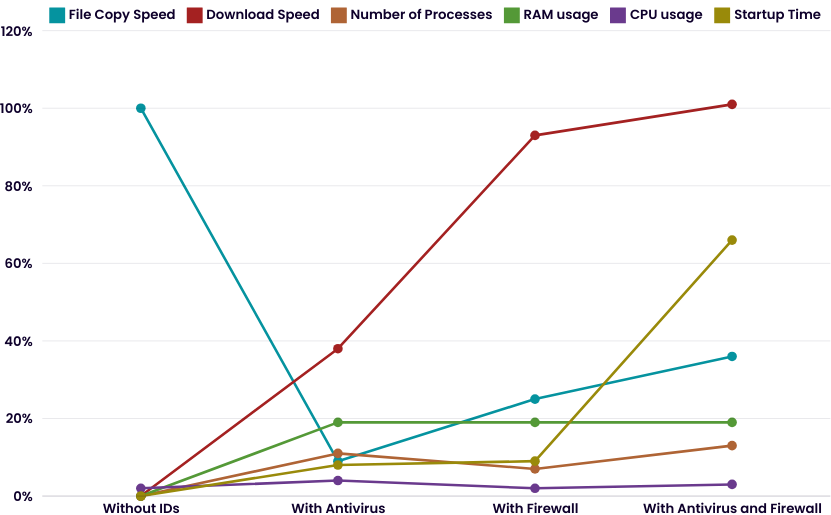
\includegraphics[width=0.9\textwidth]{resources/benchamrking_results.png}
  \caption{Impact of Antivirus and Firewall on Computational Resources}
  \label{fig:impact}
\end{figure}

\par As we can see from the figure, one of the most impacted resources is the
file copying speed, due to the fact that the antivirus and firewall scan each
file that is copied.
\par The startup time is also significantly impacted by the antivirus and
firewall, as they have to start up with the system and scan all the files that
are loaded during the startup process. Using both an antivirus and a firewall
added an extra 30s (66\%) to the startup time.
\par The download speed was faster with the antivirus and firewall installed
than with no antivirus or firewall installed. This might be due to the network
speed, as the download speed was tested by downloading a file from the internet.
\par The number of processes, RAM usage, and CPU usage were slightly impacted
by the antivirus and firewall, but the difference was not significant. This
might be due to the fact that the system had enough resources to handle the
additional processes and memory usage.

% =========================================================================== %

\section{Conclusion}
\label{sec:conclusion}

\par In conclusion, the antivirus and firewall have some impact on the
computational resources of the system, but the impact is not as significant as
expected. The file copying speed and startup time are the most impacted
resources, while the download speed, number of processes, RAM usage, and CPU
usage are slightly impacted. However, the results may not be generalizable to
all computer systems, as the performance of a computer can be influenced by
many factors, such as the hardware configuration, the operating system, and the
software installed on the system.

% =========================================================================== %

% \section{Related Work}
% \label{sec:relatedwork}

% \section{LaTeX Hints}
% \label{sec:latexhints}

% % Required for proper example rendering in the compiled PDF
% \newcount\LTGbeginlineexample
% \newcount\LTGendlineexample
% \newenvironment{ltgexample}%
% {\LTGbeginlineexample=\numexpr\inputlineno+1\relax}%
% {\LTGendlineexample=\numexpr\inputlineno-1\relax%
% %
% \tcbinputlisting{%
%   listing only,
%   listing file=\currfilepath,
%   colback=green!5!white,
%   colframe=green!25,
%   coltitle=black!90,
%   coltext=black!90,
%   left=8mm,
%   title=Corresponding \LaTeX{} code of \texttt{\currfilepath},
%   listing options={%
%     frame=none,
%     language={[LaTeX]TeX},
%     escapeinside={},
%     firstline=\the\LTGbeginlineexample,
%     lastline=\the\LTGendlineexample,
%     firstnumber=\the\LTGbeginlineexample,
%     basewidth=.5em,
%     aboveskip=0mm,
%     belowskip=0mm,
%     numbers=left,
%     xleftmargin=0mm,
%     numberstyle=\tiny,
%     numbersep=8pt%
%   }
% }
% }%

% This section contains hints on writing LaTeX.
% It focuses on minimal examples, which can be directly adapted to the content

% \subsection{Handling of paragraphs}

% \begin{ltgexample}
% One sentence per line.
% This rule is important for the usage of version control systems.
% A new line is generated with a blank line.
% As you would do in Word:
% New paragraphs are generated by pressing enter.
% In LaTeX, this does not lead to a new paragraph as LaTeX joins subsequent lines.
% In case you want a new paragraph, just press enter twice (!).
% This leads to an empty line.
% In word, there is the functionality to press shift and enter.
% This leads to a hard line break.
% The text starts at the beginning of a new line.
% In LaTeX, you can do that by using two backslashes (\textbackslash\textbackslash).\\
% This is rarely used.

% Please do \textit{not} use two backslashes for new paragraphs.
% For instance, this sentence belongs to the same paragraph, whereas the last one started a new one.
% A long motivation for that is provided at \url{http://loopspace.mathforge.org/HowDidIDoThat/TeX/VCS/#section.3}.
% \end{ltgexample}

% \subsection{Notes separated from the text}

% The package mindflow enables writing down notes and annotations in a way so that they are separated from the main text.

% \begin{ltgexample}
% \begin{mindflow}
% This is a small note.
% \end{mindflow}
% \end{ltgexample}

% \subsection{Hyphenation}

% \LaTeX{} automatically hyphenates words.
% When using microtype, there should be less hypnetations than in other settings.
% It might be necessary to tweak the hyphenations nevertheless.
% Here are some hints:

% \begin{ltgexample}
% In case you write \enquote{application-specific}, then the word will only be hyphenated at the dash.
% You can also write \verb1applica\allowbreak{}tion-specific1 (result: applica\allowbreak{}tion-specific), but this is much more effort.

% You can now write words containing hyphens which are hyphenated at other places in the word.
% For instance, \verb1application"=specific1 gets application"=specific.
% This is enabled by an additional configuration of the babel package.
% \end{ltgexample}

% \subsection{Typesetting Units}

% \begin{ltgexample}
% Numbers can be written plain text (such as 100), by using the siunitx package as follows:
% \SI{100}{\km\per\hour},
% or by using plain \LaTeX{} (and math mode):
% $100 \frac{\mathit{km}}{h}$.
% \end{ltgexample}

% \begin{ltgexample}
% \SI{5}{\percent} of \SI{10}{kg}
% \end{ltgexample}

% \begin{ltgexample}
% Numbers are automatically grouped: \num{123456}.
% \end{ltgexample}

% \subsection{Surrounding Text by Quotes}

% \begin{ltgexample}
% Please use the \enquote{enquote command} to quote something.
% Quoting with "`quote"' or ``quote'' also works.

% \end{ltgexample}

% \subsection{Cleveref examples}
% \label{sec:ex:cref}

% Cleveref demonstration: Cref at beginning of sentence, cref in all other cases.

% \begin{figure}
%     \centering
%     \includegraphics[width=.75\linewidth]{example-image-a}
%     \caption{Example figure for cref demo}
%     \label{fig:ex:cref}
% \end{figure}

% \begin{table}
%     \centering
%     \begin{tabular}{ll}
%       \toprule
%       Heading1 & Heading2 \\
%       \midrule
%       One      & Two      \\
%       Thee     & Four     \\
%       \bottomrule
%     \end{tabular}
%     \caption{Example table for cref demo}
%     \label{tab:ex:cref}
% \end{table}

% \begin{ltgexample}
% \Cref{fig:ex:cref} shows a simple fact, although \cref{fig:ex:cref} could also show something else.

% \Cref{tab:ex:cref} shows a simple fact, although \cref{tab:ex:cref} could also show something else.

% \Cref{sec:ex:cref} shows a simple fact, although \cref{sec:ex:cref} could also show something else.
% \end{ltgexample}

% \subsection{Figures}

% \begin{ltgexample}
% \Cref{fig:label} shows something interesting.

% \begin{figure}
%   \centering
%   \includegraphics[width=.8\linewidth]{example-image-golden}
%   \caption[Simple Figure]{Simple Figure. Based on \citet{mwe}.}
%   \label{fig:label}
% \end{figure}
% \end{ltgexample}

% One can also have pictures floating inside text:
% \clearpage

% \begin{ltgexample}
% \begin{floatingfigure}{.33\linewidth}
% \includegraphics[width=.29\linewidth]{example-image-a}
% \caption{A floating figure}
% \end{floatingfigure}
% \blindtext[2]
% \end{ltgexample}

% \subsection{Sub Figures}

% An example of two sub figures is shown in \cref{fig:two_sub_figures}.

% \begin{ltgexample}
% \begin{figure}[!b]
%     \centering
%     \subfloat[Case I]{\includegraphics[width=.4\linewidth]{example-image-a}%
%     \label{fig:first_case}}
%   \hfil
%     \subfloat[Case II]{\includegraphics[width=.4\linewidth]{example-image-b}%
%     \label{fig:second_case}}
%   \caption{Example figure with two sub figures.}
%   \label{fig:two_sub_figures}
% \end{figure}
% \end{ltgexample}

% \subsection{Tables}

% \begin{ltgexample}
% \begin{table}
%   \caption{Simple Table}
%   \label{tab:simple}
%   \centering
%   \begin{tabular}{ll}
%     \toprule
%     Heading1 & Heading2 \\
%     \midrule
%     One      & Two      \\
%     Thee     & Four     \\
%     \bottomrule
%   \end{tabular}
% \end{table}
% \end{ltgexample}

% \begin{ltgexample}
% % Source: https://tex.stackexchange.com/a/468994/9075
% \begin{table}
% \caption{Table with diagonal line}
% \label{tab:diag}
% \begin{center}
% \begin{tabular}{|l|c|c|}
% \hline
% \diagbox[width=10em]{Diag\\Column Head I}{Diag Column\\Head II} & Second & Third \\
% \hline
% & foo & bar \\
% \hline
% \end{tabular}
% \end{center}
% \end{table}
% \end{ltgexample}


% \subsection{Source Code}

% \begin{ltgexample}
% \Cref{lst:XML} shows source code written in XML.
% \Cref{line:comment} contains a comment.

% \begin{lstlisting}[
%   language=XML,
%   caption={Example XML Listing},
%   label={lst:XML}]
% <listing name="example">
%   <!-- comment --> (* \label{line:comment} *)
%   <content>not interesting</content>
% </listing>
% \end{lstlisting}
% \end{ltgexample}

% One can also add \verb+float+ as parameter to have the listing floating.
% \Cref{lst:flXML} shows the floating listing.

% \begin{ltgexample}
% \begin{lstlisting}[
%   % one can adjust spacing here if required
%   % aboveskip=2.5\baselineskip,
%   % belowskip=-.8\baselineskip,
%   float,
%   language=XML,
%   caption={Example XML listing -- placed as floating figure},
%   label={lst:flXML}]
% <listing name="example">
%   Floating
% </listing>
% \end{lstlisting}
% \end{ltgexample}

% One can also typeset JSON as shown in \cref{lst:json}.

% \begin{ltgexample}
% \begin{lstlisting}[
%   float,
%   language=json,
%   caption={Example JSON listing -- placed as floating figure},
%   label={lst:json}]
% {
%   key: "value"
% }
% \end{lstlisting}
% \end{ltgexample}

% Java is also possible as shown in \cref{lst:java}.

% \begin{ltgexample}
% \begin{lstlisting}[
%   caption={Example Java listing},
%   label=lst:java,
%   language=Java,
%   float]
% public class Hello {
%     public static void main (String[] args) {
%         System.out.println("Hello World!");
%     }
% }
% \end{lstlisting}
% \end{ltgexample}

% \subsection{Itemization}

% One can list items as follows:

% \begin{ltgexample}
% \begin{itemize}
% \item Item One
% \item Item Two
% \end{itemize}
% \end{ltgexample}


% One can enumerate items as follows:

% \begin{ltgexample}
% \begin{enumerate}
%   \item Item One
%   \item Item Two
% \end{enumerate}
% \end{ltgexample}


% With paralist, one can even have all items typset after each other and have them clean in the tex document:

% \begin{ltgexample}
% \begin{inparaenum}
%   \item All these items...
%   \item ...appear in one line
%   \item This is enabled by the paralist package.
% \end{inparaenum}
% \end{ltgexample}

% \subsection{Other Features}

% \begin{ltgexample}
% The words \enquote{workflow} and \enquote{dwarflike} can be copied from the PDF and pasted to a text file.
% \end{ltgexample}

% \begin{ltgexample}
% The symbol for powerset is now correct: $\powerset$ and not a Weierstrass p ($\wp$).

% $\powerset({1,2,3})$
% \end{ltgexample}

% \begin{ltgexample}
% Brackets work as designed:
% <test>
% One can also input backquotes in verbatim text: \verb|`test`|.
% \end{ltgexample}


% \section{Conclusion and Outlook}
% \label{sec:outlook}
% \lipsum[1-2]

% \subsubsection*{Acknowledgments}

% Identification of funding sources and other support, and thanks to individuals and groups that assisted in the research and the preparation of the work should be included in an acknowledgment section, which is placed just before the reference section in your document \cite{acmart}.

% %%% ===============================================================================
% %%% Bibliography
% %%% ===============================================================================

% In the bibliography, use \texttt{\textbackslash textsuperscript} for \enquote{st}, \enquote{nd}, \ldots:
% E.g., \enquote{The 2\textsuperscript{nd} conference on examples}.
% When you use \href{https://www.jabref.org}{JabRef}, you can use the clean up command to achieve that.
% See \url{https://help.jabref.org/en/CleanupEntries} for an overview of the cleanup functionality.

\renewcommand{\bibsection}{\section*{References}} % requried for natbib to have "References" printed and as section*, not chapter*
% Use natbib compatbile splncs04nat style.
% It does provide all features of splncs04.bst, but is developed in a clean way.
% Source: https://github.com/tpavlic/splncs04nat
\bibliographystyle{splncs04nat}
\begingroup
  \microtypecontext{expansion=sloppy}
  \small % ensure correct font size for the bibliography
  \bibliography{paper}
\endgroup

% Enfore empty line after bibliography
\ \\
%
All links were last followed on October 5, 2020.

%%% ===============================================================================
%\appendix
%\addcontentsline{toc}{chapter}{APPENDICES}

%\listoffigures
%\listoftables
%%% ===============================================================================

%%% ===============================================================================
%\section{My first appendix}\label{sec:appendix1}
%%% ===============================================================================
\end{document}
